%
% 4-residuen.tex -- Residuen
%
% (c) 2025 Prof Dr Andreas Müller
%
\section{Reelle Integrale mit dem cauchyschen Integralsatz
\label{buch:integration:section:residuen}}
\kopfrechts{Reelle Integrale mit dem cauchyschen Integralsatz}
Der cauchysche Integralsatz ermöglicht, reelle Integrale zu berechnen,
denen allein mit den Mitteln der reellen Analysis nur schwer beizukommen
ist.
Die Vorgehensweise ist dabei immer die Gleiche.
Das Integrationsintervall ist eine Strecke in der komplexen Ebene.
Sie wird durch weitere Wegstücke zu einem geschlossenen Weg
vervollständigt.
Die zusätzlichen Wegstücke werden so gewählt, dass sie sich
einfach berechnen lassen.
Das Integral über den geschlossenen Weg kann auch mit dem Cauchy-Integralsatz
bestimmt werden, das gesuchte Integral ergibt sich dann aus der Differenz.

%
% 41-beispiel.tex -- Ein einführendes Beispiel
%
% (c) 2026 Prof Dr Andreas Müller
%
\subsection{Ein einführendes Beispiel
\label{buch:integration:residuen:section:beispiel}}
%
% cauchy-verteilung.tex
%
% (c) 2026 Prof Dr Andreas Müller
%
\begin{figure}
\centering
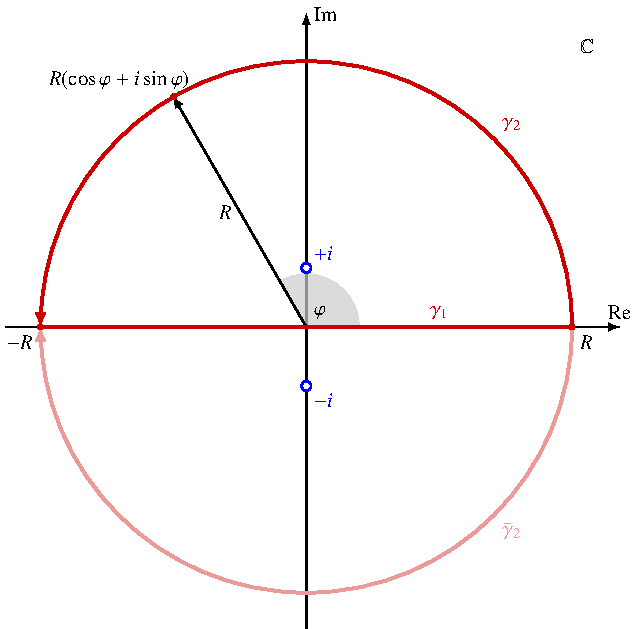
\includegraphics{chapters/030-integration/images/cauchyverteilung.pdf}
\caption{Integrationsweg für die Berechnung der Integrale
\eqref{buch:integration:residuen:eqn:cauchyintegral}
und
\eqref{buch:integration:residuen:eqn:ecos}.
\label{buch:integration:residuen:fig:cauchyverteilung}}
\end{figure}
%
Als einführendes Beispiel betrachten wir die Berechnung des uneigentlichen
Integrals
\index{uneigentliches Integral}%
\index{Integral!uneigentlich}%
\begin{equation}
I
=
\int_{-\infty}^\infty \frac{1}{x^2+1} \,dx.
\label{buch:integration:residuen:eqn:cauchyintegral}
\end{equation}
Es tritt zum Beispiel auf bei der Berechnung der Normierungskonstanten
der Cauchy-Verteilung, die die Wahrscheinlichkeitsdichte
\[
\varphi(x)
=
\frac{1}{\pi\gamma
\biggl(
\displaystyle
1+\biggl(\frac{x-x_0}{\gamma}\biggr)^2
\biggr)}
\]
hat.
Der Erwartungswert dieser Verteilung ist $x_0$, die Varianz und allere
höheren Momente sind nicht definiert.
\index{Verteilung}%
\index{Erwartungswert}%
Die $t$-Verteilung mit einem Freiheitsgrad ist ein Cauchy-Verteilung.
\index{Cauchy-Verteilung}%
\index{Verteilung!Cauchy-}%

%
% Berechnung mit der Stammfunktion
%
\subsubsection{Berechnung mit der Stammfunktion}
Zur Berechnung des
Integrals~\eqref{buch:integration:residuen:eqn:cauchyintegral}
kann natürlich die Stammfunktion verwendet werden, die in diesem
Fall einfach zu berechnen ist.
Es gilt nämlich
\[
\frac{d}{dx}\arctan(x)
=
\frac{1}{x^2 + 1}.
\]
Daher ist das Integral
\[
\int_a^a
\frac{1}{x^2+1}
\,dx
=
\Bigl[
\arctan(x)
\Bigr]_{-a}^a
=
\arctan(a) - \arctan(-a).
\]
Für das
Integral~\eqref{buch:integration:residuen:eqn:cauchyintegral}
muss der Grenzwert $a\to\infty$ berechnet werden, der
\[
\int_{-\infty}^\infty \frac{1}{x^2+1} \,dx
=
\lim_{a\to\infty}
\bigl(
\arctan(a) -\arctan(-a)
\bigr)
=
\lim_{a\to\infty} 2\arctan(a)
=
2\cdot\frac{\pi}2
=
\pi
\]
ist.

%
% Berechnung mit einem Wegintegral
%
\subsubsection{Berechnung mit einem Wegintegral}
Die Funktion
\[
z
\mapsto
f(z)
=
\frac{1}{z^2 + 1}
=
\frac1{2i}
\biggl(
\frac{1}{z-i}
-
\frac{1}{z+i}
\biggr)
\]
ist ganz offensichtlich eine holomorphe Funktion, die überall in der
komplexen Ebene ausser in den Punkten $\pm i$ definiert ist.

Ein Wegintegral entlang eines Weges, der den Punkt $+i$ umläuft,
aber nicht den Punkt $-i$,
hat den Wert
\begin{align*}
\oint_\gamma f(z)\,dz
&=
\frac1{2i}
\oint_\gamma \frac{1}{z-i}
\,dz
-
\frac1{2i}
\oint_\gamma \frac{1}{z+i}
\,dz.
\intertext{Da die Kurve den Punkt $-i$ nicht umläuft, verschwindet
das zweite Integral.
Das erste Integral kann
durch ein Integral eines 
kleinen Kreises mit der Parameterdarstellung $\gamma(t)=i+r e^{2\pi it}$
um den Punkt $+i$ ersetzt werden und ergibt}
&=
\frac{1}{2i}
\int_0^1
\frac{1}{(i+e^{2\pi it})-i}
2\pi i e^{2\pi it}\,dt
\\
&=
\frac{1}{2i}
\cdot
2\pi i
\int_0^1 
\,dt
=
\pi.
\end{align*}

Das
Integral~\eqref{buch:integration:residuen:eqn:cauchyintegral}
muss jetzt mit einem konkret gewählten Weg berechnet werden.
Dazu wählen wir den in
Abbildung~\ref{buch:integration:residuen:fig:cauchyverteilung}
dargestellten Weg.
Er führt erst als $\gamma_1$ der $x$-Achse entlang von $-R$ bis
zum Punkt $R$ und dann als $\gamma_2$ in einem grossen Halbkreis
vom Radius $R$ um den Nullpunkt wieder zurück zu $-R$.
Als Parametrisierungen für diese Wege kann man
\[
\begin{aligned}
\gamma_1(x)
&=x&
&\qquad&
&\text{für $-R\le x \le R$},
\\
\gamma_2(\varphi)
&=Re^{i\varphi}=R(\cos\varphi+i\sin\varphi)&
&\qquad&
&\text{für $0\le \varphi\le \pi$}
\end{aligned}
\]
verwenden.
Das Integral über diesen Pfad setzt sich zusammen aus den Integralen
über die beiden Teilpfade:
\begin{equation}
\begin{aligned}
\pi
=
\oint_\gamma f(z)\,dz
&=
\int_{\gamma_1} f(z)\,dz
+
\int_{\gamma_2} f(z)\,dz
\\
&=
\int_{-R}^R \frac{1}{z^2+1} \,dz
+
\int_0^{\pi} \frac{1}{R^2e^{2i\varphi}+1}\cdot iRe^{i\varphi}\,d\varphi.
\end{aligned}
\label{buch:integration:residuen:beispiel:eqn:cauchypfade}
\end{equation}
Das erste Integral konvergiert für $R\to\infty$ gegen das gesuchte
Integral~\eqref{buch:integration:residuen:eqn:cauchyintegral},
es ist also nur noch zu überlegen, was der Grenzwert des zweiten
Integrals für $R\to\infty$ ist.

Wegen
\[
\biggl|
\frac{1}{R^2e^{2i\varphi}+1}
\biggr|
=
\frac{1}{|R^2e^{2i\varphi}+1|}
\le
\frac{1}{R^2-1}
\]
folgt
\begin{align*}
\int_0^{\pi}
\frac{1}{R^2e^{2i\varphi}+1}\cdot iRe^{i\varphi}
\,d\varphi
&\le
\int_0^{\pi}
\frac{R}{R^2-1}
\,d\varphi
=
\frac{\pi R}{R^2-1}.
\end{align*}
Der Grenzwert auf der rechten Seite für $R\to\infty$ ist $0$, das
Integral über $\gamma_2$ trägt also nichts bei.
Somit folgt
\[
\pi 
=
\int_{-\infty}^\infty \frac{1}{x^2+1}\,dx,
\]
das selbe Resultat, wie wir mit der Stammfunktion gefunden haben.

%
% Ein mit der Stammfunktion nicht lösbares Beispiel
%
\subsubsection{Ein mit der Stammfunktion nicht lösbares Beispiel}
Wir wollen das Integral
\begin{equation}
\int_{-\infty}^\infty
\frac{\cos tx}{x^2+1}
\,dx
\label{buch:integration:residuen:eqn:ecos}
\end{equation}
für $t>0$ berechnen.
Es tritt zum Beispiel bei der Berechnung des Erwartungswertes 
$E(\cos(X))$ einer Cauchy-verteilten Zufallsvariable $X$ auf.
Um es mit der oben skizzierten Methode berechnen zu können,
müssen wir den Integranden erst in eine holomorphe Funktion
umwandeln.
Der Kosinus ist der Realteil $\cos x = \operatorname{Re}e^{itx}$,
auf der reellen Achse gilt also
\[
\frac{\cos x}{x^2+1}
=
\operatorname{Re}\frac{e^{itx}}{x^2+1}
\qquad
\text{für $x\in\mathbb{R}$}.
\]
Zur Berechnung des Integrals~\eqref{buch:integration:residuen:eqn:ecos}
können wir also die holomorphe Funktionen
\begin{equation}
f(z)
=
\frac{e^{itz}}{z^2+1}
\end{equation}
verwenden.

Mit dem gleichen Weg
\eqref{buch:integration:residuen:beispiel:eqn:cauchypfade}
wie vorhin können wir versuchen, das Integral
\begin{align*}
\oint_\gamma
\frac{e^{itz}}{z^2+1}
\,dz
&=
\oint_\gamma
\frac{e^{itz}}{2i}
\biggl(
\frac{1}{z-i}
-
\frac{1}{z+i}
\biggr)
\,dz
=
\oint_\gamma
\frac{e^{itz}}{2i}
\biggl(
\frac{1}{z-i}
\,dz
-
\oint_\gamma
\frac{1}{z+i}
\biggr)
\,dz.
\intertext{mit Hilfe des Integralsatzes zu berechnen.
Der Weg $\gamma$ dreht sich einmal um den Punkt $i$, nicht aber um $-i$.
Es bleibt also nur das erste Integral}
&=
\frac{1}{2i}
\oint_\gamma
\frac{e^{itz}}{z-i}
\,dz
=
\pi\cdot 
\frac{1}{2\pi i}
\oint_\gamma
\frac{e^{itz}}{z-i}
\,dz
\intertext{welches nach dem Integralsatz durch den Wert des Zählers
an der Stelle $z=i$ ersetzt werden kann:}
&=
\pi \cdot e^{it\cdot i}
=
\pi e^{-t}.
\end{align*}
Um zu zeigen, dass dies
der gesuchte Wert des Integrals ist, müssen wir den Weg wieder in
die beiden Teile $\gamma_1$ und $\gamma_2$ zerlegen.
\begin{align*}
\oint_\gamma
\frac{e^{itz}}{z^2+1}
\,dz
&=
\int_{-R}^R
\frac{e^{itx}}{x^2+1}
\,dx
+
\int_0^1
\frac{e^{it\gamma_2(t)}}{\gamma_2(t)^2+1}
\,dt.
\end{align*}
Das erste Integral konvergiert für $R\to\infty$ gegen das gesuchte
Integral, wir müssen also nur noch zeigen, dass das zweite Integral
keinen Beitrag leistet.
Dazu müssen wir den Integranden mit Hilfe der Parametrisierung
\[
\gamma_2(\varphi)=R(\cos\varphi+i\sin\varphi)
\qquad\Rightarrow\qquad
|\gamma_2(\varphi)|
=
R
\]
abschätzen:
\begin{align}
\biggl|\frac{e^{itz}}{z^2+1}\biggr|
&=
\frac{|e^{itz}|}{|z^2+1|}
\le
\frac{|e^{itR(\cos \varphi + i\sin\varphi)}|}{|z|^2+1}
=
\frac{|e^{itR\cos\varphi}|\cdot e^{-tR\sin\varphi}}{R^2+1}
\le
\frac{1}{R^2+1}
\label{buch:integration:residuen:bsp:abschaetzung}
\end{align}
Wie im früheren Beispiel folgt
\begin{align*}
\biggl|
\int_{\gamma_2} \frac{e^{itz}}{z^2+1}\,dz
\biggr|
&=
\biggl|
\int_{\gamma_2}
\frac{e^{it\gamma_2(\varphi)}}{\gamma_2(\varphi)^2+1}
\dot\gamma_2(\varphi)
\,d\varphi
\biggr|
\le
\int_0^\pi \frac{1}{R^2+1} R \,dt
=
\frac{\pi R}{R^2+1}.
\end{align*}
Die rechte Seite konvergiert für $R\to\infty$ gegen $0$ und es folgt
\begin{equation}
\int_{-\infty}^\infty
\frac{\cos xt}{x^2+1}
\,dx
=
\operatorname{Re}
\oint_\gamma \frac{e^{itz}}{z^2+1}\,dz
=
\pi e^{-t}
\qquad
\text{für $t\ge 0$}.
\label{buch:integration:residuen:eqn:pie-t}
\end{equation}
Damit ist das Integral berechnet.
Man beachte, dass für diesen Integranden keine Stammfunktion
gefunden werden kann, die vorgestellte Methode ist also die einzige
Methode zur Berechnung des Integrals.

Das Integral
\eqref{buch:integration:residuen:eqn:ecos}
kann auch für $t\ge 0$ berechnet werden.
Die Schwierigkeit besteht darin, dass die obere Schranke der Abschätzung
\eqref{buch:integration:residuen:bsp:abschaetzung}
exponentiell anwächst.
Man muss daher den an der reellen Achse gespiegelten Weg mit der
Parametrisierung
\[
\gamma_2(\varphi)
=
R(\cos\varphi - i\sin\varphi)
\]
verwenden.
Die Abschätzung wird dann
\[
\biggl|
\frac{e^{itz}}{z^2+1}
\biggr|
\le
\frac{|e^{itR\cos\varphi}|\cdot e^{tR\sin\varphi}}{R^2+1}
\le
\frac{1}{R^2+1}.
\]
Der gespiegelt Weg läuft nicht mehr um den Punkt $i$, sondern um den
Punkt $-i$, und er umläuft ihn im Uhrzeigersinn.
Es folgt daher
\begin{align*}
\oint_\gamma
\frac{e^{itz}}{z^2+1}
\,dz
&=
\pi
\frac{1}{2\pi i}
\oint_{\gamma}
-
\frac{e^{itz}}{z+i}
\,dz
=
\pi e^{t}
\end{align*}
und daher erneut
\begin{equation}
\int_{-\infty}^\infty
\frac{\cos tx}{x^2 + 1}
\,dx
=
\pi e^{t}
\qquad
\text{für $t<0$}.
\label{buch:integration:residuen:eqn:piet}
\end{equation}

Die Resultate
\eqref{buch:integration:residuen:eqn:pie-t}
und
\eqref{buch:integration:residuen:eqn:piet}
unterscheiden sich nur durch das Vorzeichen in der Exponentialfunktion,
man kann dies auch schreiben als
\[
\int_{-\infty}^\infty
\frac{\cos tx}{x^2+1}
\,dx
=
\begin{cases}
\pi e^{-t}&\qquad \text{für $t \ge 0$}\\
\pi e^{t} &\qquad \text{für $t < 0$}.
\end{cases}
\]
Die Fallunterscheidung
\[
\begin{cases}
         - t&\qquad \text{für $t \ge 0$}\\
\phantom{-}t&\qquad \text{für $t \le 0$}
\end{cases}
\]
liefert immer eine negative Zahl vom Betrag $t$, in der Tat ist
\[
|t|
=
\begin{cases}
         - t&\qquad \text{für $t \ge 0$}\\
\phantom{-}t&\qquad \text{für $t \le 0$}.
\end{cases}
\]
Damit kann man jetzt auch die Resultate
\eqref{buch:integration:residuen:eqn:pie-t}
und
\eqref{buch:integration:residuen:eqn:piet}
zu
\begin{equation}
\int_{-\infty}^\infty
\frac{\cos tx}{x^2 + 1}
\,dx
=
\pi e^{-|t|}
\end{equation}
zusammenfassen.
Tatsächlich ändert der Integrand nicht, wenn man $t$ durch $-t$ ersetzt.

%
% 42-methode.tex -- Die Methode
%
% (c) 2026 Prof Dr Andreas Müller
%
\subsection{Die Methode}
Die im Abschnitt~\ref{buch:integration:residuen:section:beispiel}
dargestellt Methode löst also die Aufgabe ein reelles Integral
%
% fig-methode.tex
%
% (c) 2026 Prof Dr Andreas Müller
%
\begin{figure}
\centering
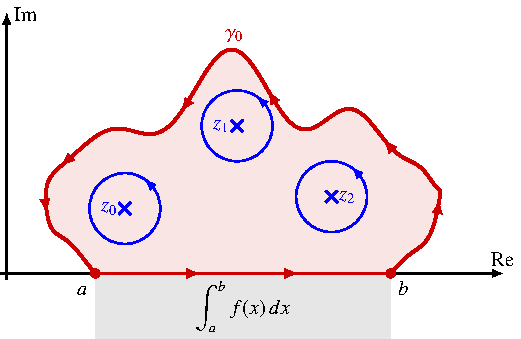
\includegraphics{chapters/030-integration/images/methode.pdf}
\caption{Die komplexe Wegintegration ermöglicht das Integral der
reellen Funktion $f(x)$ durch ein Integral einer geeigneten
komplexen Funktion $f(z)$ entlang des Weges
$\gamma_0$ und auszudrücken.
Falls im Inneren des roten Gebietes Singularitäten der Funktion $f(z)$
auftreten, symbolisiert durch die blauen Punkte, dann kommen 
noch Kurvenintegrale entlang kleinen Kreisen um die Singularitäten
hinzu.
\label{buch:integration:residuen:fig:methode}}
\end{figure}
%
\[
I
=
\int_a^b f(x)\,dx
\]
zu lösen.
Sie geht dazu wie folgt vor.

\begin{enumerate}
\item
Die reelle Funktion im Integranden muss durch eine komplexe
Funktion $f(z)$ ersetzt werden.
\item
Das Integral entlang des Segmentes $[a,b]$ auf der reellen Achse
wird durch ein Kurve $\gamma_0$ zu einem geschlossenen Weg $\gamma$
ergänzt, wie er in
Abbildung~\ref{buch:integration:residuen:fig:methode}
dargestellt ist.
\item
Falls der Integrand im Inneren der Kurve $\gamma$ holomorph ist,
verschwindet das Wegintegral.
Dann folgt, dass das Integral durch
\[
I
=
\int_a^b f(x)\,dx
=
-\int_{\gamma_0} f(z)\,dz
\]
berechnet werden kann.
\item
Falls im Inneren der Kurve $\gamma$ Singularitäten des Integranden
vorhanden sind (in der Abbildung~\ref{buch:integration:residuen:fig:methode}
durch blaue Kreuze dargestellt), muss diesen durch zusätzliche
Summanden auf der rechten Seite Rechnung getragen werden.
\index{Singularitat@Singularität}%
Da dies durch Integrale über beliebig kleine Kreise um die Singularitäten
herum geschehen kann, hängen diese Korrekturterme nur von den
Funktionswerten und Ableitungen in unmittelbarer Nähe der
Singularität ab.
Techniken zu ihrer Berechnung, insbesondere der Begriff des Residuums,
\index{Residuum}%
werden in Kapitel~\ref{chapter:analytisch} dargestellt.
Das Integral ist dann
\[
\int_a^b f(x)\,dx
=
-\int_{\gamma_0} f(z)\,dz
+
\text{Singularitätenterme.}
\]
\end{enumerate}
Da die Berechnung der Singularitätenterme, wie im einführenden Beispiel,
meist nicht schwierig ist, ist die Methode vor allem dann erfolgreich,
wenn das Wegintegral entlang $\gamma_0$ deutlich einfacher zu berechnen
ist.

Die Methode wird oft in Fällen angewendet, wo der Weg von einem
Parameter abhängt, wie im einführenden Beispiel der Radius $R$.
Wenn der gesuchte Integralwert ein Grenzwert für den Parameter ist,
kann man hoffen, dass das Integral über $\gamma_0$ im Grenzwert
deutlich einfacher zu berechnen ist.
Im Beispiel ist das Integral über den zusätzlichen Wegteil im
Grenzwert sogar verschwunden.

Im nächsten Abschnitt wird ein weiteres Beispiel für diese Methode
gezeigt. 
Ausserdem motiviert die Methode auch den Begriff des Hauptwertes,
der in Abschnitt~\ref{buch:integration:residuen:subsection:hauptwert}
skizziert und in Kapitel~\ref{chapter:hauptwert} ausführlicher
erklärt wird.

%
% 43-pole.tex -- Ein Beispiel ohne Pole
%
% (c) 2026 Prof Dr Andreas Müller
%
\subsection{Ein Beispiel ohne Pole}
%
% fig-ecos.tex
%
% (c) 2026 Prof Dr Andreas Müller
%
\begin{figure}
\centering
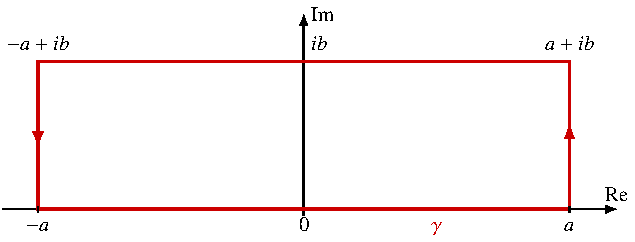
\includegraphics{chapters/030-integration/images/ecos.pdf}
\caption{Weg zur Auswertung des Integrals
$\int_{-\infty}^\infty \cos 2bx \cdot e^{-x^2}\,dx$.
\label{buch:integration:residuen:fig:ecos}}
\end{figure}
%
Die Funktion $f(z)=e^{-z^2}$ ist holomorph in der ganzen komplexen 
Ebene, für jeden beliebigen geschlossenen Weg gilt daher nach dem
Satz~\ref{buch:integration:wegintegral:satz:cauchy}
von Cauchy
\begin{equation}
\int_{\gamma} e^{-z^2}\,dz
=
0.
\label{buch:integration:residuen:eqn:wegintegral}
\end{equation}
Die Funktion $e^{-z^2}$ ist bekannt dafür, dass sie keine elementare
Stammfunktion hat.
Da sie aber in der Wahrscheinlichkeitsdichte der Normalverteilung
vorkommt, sind Integrale dieser Funktion von einiger praktischer
Bedeutung.

Das uneigentliche Integral
\index{Integral!uneigentlich}%
\[
\int_{-\infty}^{\infty} e^{-x^2}\,dx = \!\sqrt{\pi}
\]
kann mithilfe eines zweifachen Integrals bestimmt werden, wir nehmen
es hier als bekannt an.

Wir betrachten jetzt das Integral entlang des rechteckigen Weges $\gamma$
in Abbildung~\ref{buch:integration:residuen:fig:ecos}.
Das Integral über den unteren Rand des Rechtecks ist
\[
\int_{-a}^a
e^{-x^2}
\,dx
\to
\!\sqrt{\pi}
\]
für $a\to\infty$.
Wegen~\eqref{buch:integration:residuen:eqn:wegintegral}
müssen die verbleibenden Teile des Weges den Wert $-\!\sqrt{\pi}$ ergeben.
Wir berechnen diese Teile.

Die vertikalen Teile des Weges haben die Form
\begin{align*}
\int_0^b
e^{-(a+iy)^2}
\cdot i
\,dy
&=
i
e^{-a^2}
\int_0^b
e^{y^2 -2iby}
\,dy
\intertext{mit Betrag}
\biggl|
\int_0^b
e^{-(a+iy)^2}
\cdot i
\,dy
\biggr|
&=
e^{-a^2}
\biggl|
\int_0^b
e^{y^2 -2iby}
\,dy
\biggr|
\\
&\le
e^{-a^2}
\int_0^b
\bigl|e^{y^2 -2iby}\bigr|
\,dy
=
e^{-a^2}
\int_0^b
e^{y^2}
\,dy
\le
e^{-a^2}be^{b^2}.
\end{align*}
Die rechte Seite konvergiert gegen $0$, wenn $a\to\infty$.
Im Grenzwert $a\to\infty$ tragen die vertikalen Teile des Weges
also nichts bei.

Wir können jetzt schliessen, dass im Grenzwert $a\to\infty$ sich die
Integrale über den oberen und unter Rand wegheben.
Das Integral über den oberen Rand des Rechtecks ist
\begin{align*}
\int_{a}^{-a}
e^{-(x+ib)^2}
\,dx
&=
\int_{a}^{-a}
e^{-x^2+b^2-2ixb}
\,dx
=
e^{b^2}
\int_{a}^{-a}
e^{-x^2}
\bigl(
\cos(2bx) - i\sin(2bx)
\bigr)
\,dx
\\
&=
e^{b^2}
\int_{a}^{-a}
e^{-x^2}
\cos(2bx)
\,dx
-i
e^{b^2}
\int_{a}^{-a}
e^{-x^2}
\sin(2bx)
\,dx.
\end{align*}
Das zweite Integral hat einen ungeraden Integranden, wird aber über
ein symmetrisches Interval erstreckt, daher verschwindet es.
Im Grenzwert $a\to\infty$ gilt
\begin{align*}
\!\sqrt{\pi}
+
e^{b^2}
\int_{\infty}^{-\infty}
e^{-x^2}
\cos(2bx)
\,dx
&=
0
\\
\!\sqrt{\pi}
&=
e^{b^2}
\int_{-\infty}^{\infty}
e^{-x^2}
\cos(2bx)
\,dx
\intertext{oder}
\int_{-\infty}^{\infty}
e^{-x^2}
\cos(2bx)
\,dx
&=
\!\sqrt{\pi}e^{-b^2}.
\end{align*}
Man beachte, dass das Integral nicht mit der traditionellen Methode
der Stammfunktion berechnet werden kann.
Wie für den Integranden $e^{-x^2}$ kann auch für den Integranden
$\cos(2bx)e^{-x^2}$ kein Stammfunktion in geschlossener Form
gefunden werden.
Die Methode der Wegintegrale in der komplexen Ebene ist also die
einzige Methode, dieses Integral exakt zu berechnen.

%
% 44-hauptwert.tex -- Hauptwert
%
% (c) 2026 Prof Dr Andreas Müller
%
\subsection{Hauptwert
\label{buch:integration:residuen:subsection:hauptwert}}
Die Berechnung des Integrals in
Abschnitt~\ref{buch:integration:residuen:section:beispiel}
hat einen Weg verwendet, der den Nullpunkt in einem grossen
Bogen umrundet hat.
So wurde das Integral zwischen $-R$ und $R$ zu einem Wegintegral
über eine geschlossene Kurve vervollständigt, wodurch sich der
Integralsatz anwenden liess.
Auf diese Weise konnte ein uneigentliches Integral von 
$1/(x^2+1)$ über die ganze reelle Achse berechnet werden.

Auch das Integral
%
% fig-sinxx.tex
%
% (c) 2026 Prof Dr Andreas Müller
%
\begin{figure}
\centering
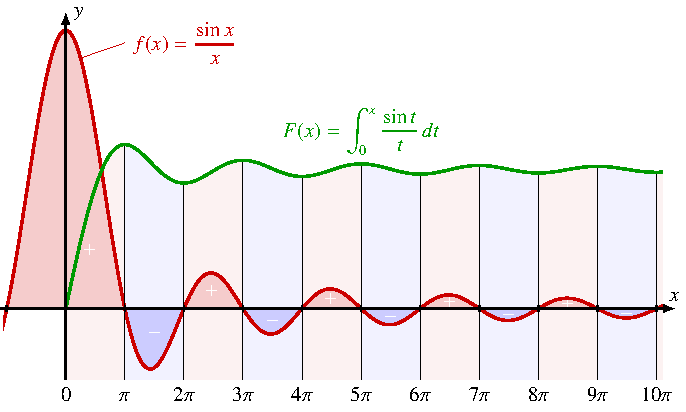
\includegraphics{chapters/030-integration/images/sinxx.pdf}
\caption{Die Stammfunktion von $f(x) = \sin(x)/x$ oszilliert, die Extrema
befinden sich bei den Nullstellen des Integranden, die ganzzahlige
Vielfache von $\pi$ sind.
\label{buch:integration:fig:sinxx}}
\end{figure}
%
\begin{equation}
I
=
\int_{-\infty}^\infty \frac{\sin x}{x}\,dx
\label{buch:integration:residuen:eqn:sinxxintegral}
\end{equation}
ist uneigentlich.
Da der Integrand mit Nullstellen bei ganzzahligen Vielfachen
von $\pi$ oszilliert, nimmt die Stammfunktion
\[
x
\mapsto
F(x)
=
\int_{0}^{x} \frac{\sin t}{t}\,dt
\]
lokale Extrema bei diesen Nullstellen an
(Abbildung~\ref{buch:integration:fig:sinxx}).
Jeder Wert liegt daher zwischen Werten
\[
F\biggl(
\biggl\lfloor\frac{x}{\pi}\biggr\rfloor\pi
\biggr)
=
\int_{0}^{\lfloor\frac{x}{\pi}\rfloor\pi}
\frac{\sin t}{t}\,dt
\qquad
\text{und}
\qquad
F\biggl(
\biggl(\biggl\lfloor\frac{x}{\pi}\biggr\rfloor+1\biggr)\pi
\biggr)
=
\int_{0}^{\left(\lfloor\frac{x}{\pi}\rfloor+1\right)\pi}
\frac{\sin t}{t}\,dt
\]
der Stammfunktion an den nächstliegenden ganzzahligen Vielfachen von $\pi$.
Die Konvergenz des uneigentlichen Integrals ist damit gesichert.
Trotzdem bleibt die Berechnung des Integralwertes offen, da es
keine geschlossene Form für die Stammfunktion gibt.

Um den Werte des Integrals $I$ mithilfe eines Wegintegrals zu berechnen,
muss ein komplexer Integrand und ein passender Weg gefunden werden.
Dabei ist zu berücksichtigen, dass der Integrand an der Stelle $x=0$
eine Singularität hat.
%
% fig-hauptwert.tex
%
% (c) 2026 Prof Dr Andreas Müller
%
\begin{figure}
\centering
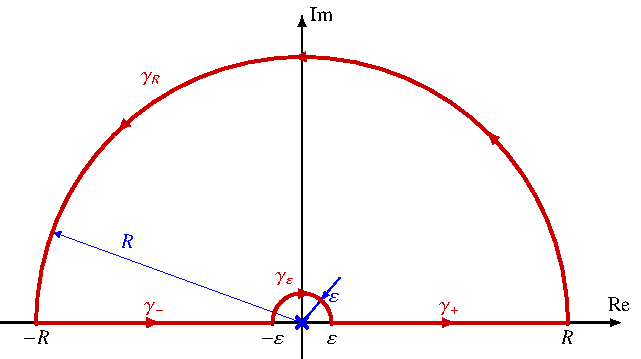
\includegraphics{chapters/030-integration/images/hauptwert.pdf}
\caption{Weg zur Berechnung des Integrals
\eqref{buch:integration:residuen:eqn:sinxxintegral}
mit Hilfe des Weges $\gamma$, der sich aus einem grossen
Kreis mit Radius $R$ und einem kleinen Kreis mit Radius
$\varepsilon$ zusammensetzt.
Dadurch wird die Singularität des Integranden $e^{iz}/z$ an der Stelle
$z=0$ gemieden.
\label{buch:integration:residuen:fig:hauptwert}}
\end{figure}
%
Als Integrand bietet sich
\[
f(z)
=
\frac{e^{iz}}{z}
\]
an.
Während der ursprüngliche reelle Integrand an der Stelle $x=0$ stetig
ist, hat $f(z)$ dort einen Pol.
Als Weg kann der in
Abbildung~\ref{buch:integration:residuen:fig:hauptwert}
dargestellte Weg verwendet werden.
Er setzt sich zusammen aus den beiden Segmenten $[\varepsilon,R]$
und $[-R,-\varepsilon]$ und den Kreisbögen $\gamma_R$ und
$\gamma_\varepsilon$ mit Radien $R$ und $\varepsilon$,
die die Segmente zu einem geschlossenen Weg verbinden.
Im Inneren dieses Weges ist $f(z)$ eine holomorphe Funktion.
Nach dem Integralstatz verschwindet das komplexe Wegintegral
\begin{equation}
\int_{\gamma_+\cdot\gamma_R\cdot\gamma_-\cdot\gamma_\varepsilon} f(z)\,dz
=
\int_{\gamma_+} f(z)\,dz
+
\int_{\gamma_R} f(z)\,dz
+
\int_{\gamma_-} f(z)\,dz
+
\int_{\gamma_\varepsilon} f(z)\,dz
=
0
\label{buch:integration:residuen:eqn:summe}
\end{equation}
über den ganzen Weg.
Das gesuchte Integral $I$ ist der Teil über die beiden Segmente
$\gamma_\pm$ im Grenzwert
\begin{align*}
I
&=
\lim_{R\to\infty}
\lim_{\varepsilon\to 0}
\biggl(
\int_{\gamma_+}
f(z)\,dz
+
\int_{\gamma_-}
f(z)\,dz
\biggr)
\intertext{für $R\to\infty$ und $\varepsilon\to 0$.
Aus \eqref{buch:integration:residuen:eqn:summe} kann man dann
schliessen, dass das Integral auch}
&=
-
\lim_{R\to\infty}
\int_{\gamma_R} f(z)\,dz
-
\lim_{\varepsilon\to 0}
\int_{\gamma_{\varepsilon}} f(z)\,dz
\end{align*}
ist.
Diese Vorgehensweise berechnet das Integral entlang der
reellen Achse mit symmetrischen Segmenten, während
die Definition eines uneigentlichen Integrals verlangt, dass für
die beden Grenzen unabhängig voneinander ein Grenzübergang durchgeführt
wird.
Der symmetrische Grenzwert heisst auch der \emph{Hauptwert} des
Integrals und wird im Kapitel~\ref{chapter:hauptwert} ausführlicher 
dargestellt.





